% Options for packages loaded elsewhere
\PassOptionsToPackage{unicode,pdfusetitle}{hyperref}
\PassOptionsToPackage{hyphens}{url}
\PassOptionsToPackage{dvipsnames,svgnames*,x11names*}{xcolor}

\documentclass[10pt,ignorenonframetext]{beamer}
\usepackage{lmodern}
\usepackage{amssymb,amsmath,mathtools,amsthm}
\usepackage[T1]{fontenc}
\usepackage[utf8]{inputenc}
\usepackage{textcomp} % provide euro and other symbols

\usepackage{pgfpages}

% prevent slide breaks in the middle of a paragraph
\widowpenalties 1 10000
\raggedbottom

% redefine part, section, and subsection headers
\raggedbottom
\setbeamertemplate{part page}{
 \centering
 \begin{beamercolorbox}[sep=16pt,center]{part title}
    \usebeamerfont{part title}\insertpart\par
 \end{beamercolorbox}
}
\setbeamertemplate{section page}{
 \centering
 \begin{beamercolorbox}[sep=12pt,center]{part title}
    \usebeamerfont{section title}\insertsection\par
 \end{beamercolorbox}
}
\setbeamertemplate{subsection page}{
 \centering
 \begin{beamercolorbox}[sep=8pt,center]{part title}
    \usebeamerfont{subsection title}\insertsubsection\par
 \end{beamercolorbox}
}

\AtBeginPart{\frame{\partpage}}
\AtBeginSection{\ifbibliography\else\frame{\sectionpage}\fi}
\AtBeginSubsection{\frame{\subsectionpage}}

% beamer configuration
\usecolortheme{dove}
\usefonttheme{professionalfonts}
\usefonttheme{structurebold}
\setbeamertemplate{footline}[frame number]
\setbeamertemplate{caption}[numbered]
\setbeamertemplate{caption label separator}{: }
\setbeamercolor{caption name}{fg=normal text.fg}
\setbeamertemplate{frametitle}{\begin{centering}\insertframetitle\par\end{centering}}
\setbeamertemplate{itemize items}[circle]
\setbeamerfont{frametitle}{size=\large}
\setbeamertemplate{headline}{\vskip5ex}
\beamertemplatenavigationsymbolsempty
%\setlength{\parskip}{1em} % add paragraph spacing

% Use upquote if available, for straight quotes in verbatim environments
\usepackage{upquote}
\usepackage[]{microtype}
\UseMicrotypeSet[protrusion]{basicmath} % disable protrusion for tt fonts

\usepackage{xcolor}
\usepackage{xurl} % add URL line breaks if available
\usepackage{bookmark}
\usepackage{hyperref}
\hypersetup{
  colorlinks=true,
  linkcolor=Maroon,
  filecolor=Maroon,
  citecolor=Blue,
  urlcolor=Blue
}

% tikz and pgfplots stuff
\usepackage{tikz}
\usetikzlibrary{arrows,shapes,positioning,intersections}
\usepackage{pgfplots}
\usepgfplotslibrary{external,colormaps}
\pgfplotsset{width=7cm,compat=1.11}
\tikzexternalize

\urlstyle{same} % disable monospaced font for URLs
\newif\ifbibliography
\setlength{\emergencystretch}{3em} % prevent overfull lines
\setcounter{secnumdepth}{-\maxdimen} % remove section numbering

%\usepackage{subfig}
\usepackage{subcaption}
\usepackage{algorithm,algpseudocode}
\usepackage{booktabs}

\DeclareMathOperator*{\argmax}{arg\,max}
\DeclareMathOperator*{\argmin}{arg\,min}
\DeclareMathOperator{\E}{\text{E}}
\DeclareMathOperator{\var}{var}
\DeclareMathOperator{\cov}{cov}
\DeclareMathOperator{\sign}{sign}
\DeclareMathOperator{\card}{card}
\DeclareMathOperator{\cumsum}{cumsum}
\DeclareMathOperator*{\prox}{prox}
\newcommand{\pkg}[1]{\textsf{#1}}
\renewcommand{\vec}{\vectorsym}
\newcommand{\mat}{\matrixsym}
\newcommand{\du}{\mathrm{d}}

% biblatex
\usepackage[citestyle=authoryear]{biblatex}
\addbibresource{references.bib}

\title{The Strong Screening Rule for SLOPE}
\subtitle{Statistical Learning Seminar}
\author[shortname]{\texorpdfstring{\alert{Johan Larsson}}{Johan Larsson}\inst{1} \and Małgorzata Bogdan\inst{1,2} \and Jonas Wallin\inst{1}}
\institute[shortinst]{\inst{1} Department of Statistics, Lund University, \and %
                      \inst{2} Department of Mathematics, University of Wroclaw}
\date{May 8, 2020}
\titlegraphic{
\includegraphics{lu.pdf}}

\begin{document}
\frame[noframenumbering,plain]{\titlepage}

% \hypertarget{first-section}{%
% \section{Setting}\label{first-section}}

\begin{frame}{Recap: SLOPE}
\protect\hypertarget{introduction}{}

The SLOPE ~\autocite{bogdan2015} estimate is 
\[
\hat\beta = \argmin_{\beta \in \mathbb{R}^p}\left\{ g(\beta) + J(\beta;\lambda) \right\}
\]
where \(J(\beta;\lambda)=\sum_{i=1}^p\lambda_i \lvert \beta \rvert_{(i)}\) is the \alert{sorted \(\ell_1\) norm},
where
\[
    \lambda_1 \geq \lambda_2 \geq \cdots \geq \lambda_p \geq 0, \qquad 
    \lvert \beta \rvert_{(1)} \geq \lvert \beta \rvert_{(2)} \geq \cdots \geq \lvert \beta \rvert_{(p)}.
\]
\medskip
\begin{columns}[T]
\begin{column}{0.45\textwidth}
Here we are interested in fitting a \alert{path} of regularization
penalties \(\lambda^{(1)}, \lambda^{(2)}, \dots, \lambda^{(m)}\)\medskip

We will
let \(\hat\beta(\lambda^{(i)})\) correspond to the solution to SLOPE at the
\(i\)th step on the path.
\end{column}
\begin{column}{0.45\textwidth}
\pgfplotsset{width=6cm,height=6cm}
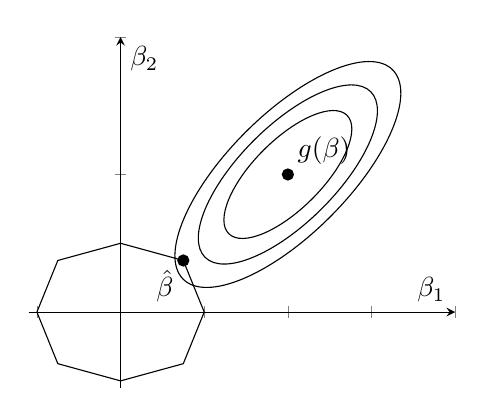
\begin{tikzpicture}
\begin{axis}[
    xlabel = \(\beta_1\),
    ylabel = \(\beta_2\),
    ymin = -1.1,
    ymax = 4,
    xmin = -1.1,
    xmax = 4,
    axis lines = center,
    yticklabels={,,},
    xticklabels={,,}
]
\draw[rotate around={45:(2,2)}] (2,2) ellipse (1 and 0.5);
\draw[rotate around={45:(2,2)}] (2,2) ellipse (1.4 and 0.7);
\draw[rotate around={45:(2,2)}] (2,2) ellipse (1.77 and 0.87);

\addplot[]
    coordinates {
    	(-1,0)
    	(-0.75, 0.75)
    	(0,1)
    	(0.75,0.75)
    	(1,0)
    	(0.75,-0.75)
    	(0,-1)
    	(-0.75,-0.75)
    	(-1,0)
    };
\addplot [only marks, mark=*] coordinates {(2,2)};
\node [above right,black] at (2,2) {$g(\beta)$};

\addplot [only marks, mark=*] coordinates { (0.75,0.75) };
\node [below left] at (0.75,0.75) {$\hat\beta$};
\end{axis}
\end{tikzpicture}   
\end{column}
\end{columns}

\end{frame}

% \begin{frame}{Problem}
% \protect\hypertarget{introduction}{}

% Solving SLOPE~\autocite{bogdan2015}
% returns optimal point \(\hat\beta\) in variable \(\beta\) to
% the optimization problem
% \[
% \begin{aligned}
%     &\text{minimize}   && g(\beta) \\
%     &\text{subject to} && \sum_{i=1}^n w_i \lvert \beta \rvert_{(i)} \leq t,
% \end{aligned}
% \]
% or equivalently (in Lagrangian form),
% \[
% \hat\beta = \argmin_{\beta \in \mathbb{R}^p}\left\{ g(\beta) + \sum_{i=1}^p \lambda_i \lvert\beta\rvert_{(i)}\right\}
% \]
% where \(\sum_{i=1}^p\lambda_i \lvert \beta \rvert_{(i)}\) is the \alert{sorted \(\ell_1\) norm},
% for which
% \[\lambda_1 \geq \lambda_2 \geq \cdots \geq \lambda_p \geq 0\]
% and
% \[\lvert \beta \rvert_{(1)} \geq \lvert \beta \rvert_{(2)} \geq \cdots \geq \lvert \beta \rvert_{(p)}.\]
% \end{frame}

% \begin{frame}{SLOPE constraint region}
% sorted \(\ell_1\) norm defines a constraint region and the solution \(\hat\beta\) is
% found at an intersection between the level curves of the smooth part, \(h\) and the
% constraint region

% \begin{center}
% 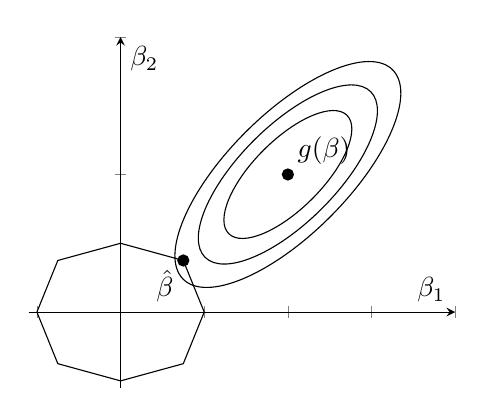
\begin{tikzpicture}
\begin{axis}[
    xlabel = \(\beta_1\),
    ylabel = \(\beta_2\),
    ymin = -1.1,
    ymax = 4,
    xmin = -1.1,
    xmax = 4,
    axis lines = center,
    yticklabels={,,},
    xticklabels={,,}
]
\draw[rotate around={45:(2,2)}] (2,2) ellipse (1 and 0.5);
\draw[rotate around={45:(2,2)}] (2,2) ellipse (1.4 and 0.7);
\draw[rotate around={45:(2,2)}] (2,2) ellipse (1.77 and 0.87);

\addplot[]
    coordinates {
    	(-1,0)
    	(-0.75, 0.75)
    	(0,1)
    	(0.75,0.75)
    	(1,0)
    	(0.75,-0.75)
    	(0,-1)
    	(-0.75,-0.75)
    	(-1,0)
    };
\addplot [only marks, mark=*] coordinates {(2,2)};
\node [above right,black] at (2,2) {$g(\beta)$};

\addplot [only marks, mark=*] coordinates { (0.75,0.75) };
\node [below left] at (0.75,0.75) {$\hat\beta$};
\end{axis}
\end{tikzpicture}    
% \end{center}
% \end{frame}

% \begin{frame}{Choosing \(\lambda\)}
% \begin{itemize}
%     \item \(\lambda\) is \(p\)-dimensional, which means there is \alert{considerable} 
%           freedom in choosing it
%     \item typically no informative decision\footnote{Except under
%           certain, in general prohibitive, assumptions} and must rely on cross-validation
%     \item to make this problem manageable, we therefore assume that each \(\lambda_i\)
%           is a function of \(p\), \(n\), \(i\), and some parameters
% \end{itemize}
% \end{frame}

% \begin{frame}{Principled choices of \(\lambda\)}
% \begin{columns}
%     \begin{column}{0.55\linewidth}
%         \begin{block}{OSCAR~\autocite{bondell2008}}
%             \[a(p - i) + b\]
%         \end{block}
%         \begin{block}{Benjamini--Hochberg (BH)~\autocite{bogdan2015}}
%             \[\sigma\Phi^{-1}\left(1 - \frac{qi}{2p}\right),\]
%             where \(\Phi^{-1}\) is the quantile function for the
%             standard normal distribution
%         \end{block}
%         \begin{block}{Gaussian~\autocite{bogdan2015}}
%             \[\min\left(\lambda_{i-1}, \lambda^{\mathrm{BH}}_i\sqrt{1 + \frac{1}{n-i} \sum_{j < i}\lambda_i^2}\right)\]
%         \end{block}
%     \end{column}
%     \begin{column}{0.45\linewidth}
%     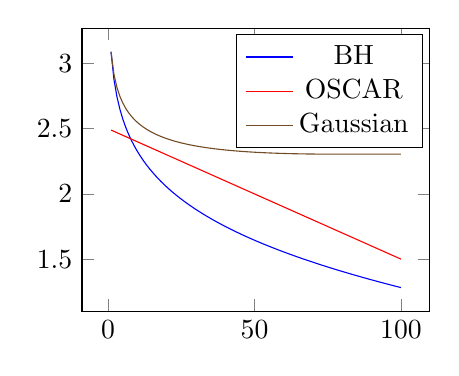
\begin{tikzpicture}
\begin{axis}[no marks,width=6cm]
    \addplot+
        coordinates {
            (1,3.090232306167818)
            (2,2.878161739095489)
            (3,2.747781385444999)
            (4,2.652069807902201)
            (5,2.5758293035489053)
            (6,2.5121443279304674)
            (7,2.457263390205441)
            (8,2.4089155458154656)
            (9,2.3656181268642973)
            (10,2.326347874040846)
            (11,2.2903678778552723)
            (12,2.25712924448623)
            (13,2.22621176931718)
            (14,2.1972863766410575)
            (15,2.170090377584565)
            (16,2.1444106209118456)
            (17,2.120071689742156)
            (18,2.0969274291643467)
            (19,2.074854734393314)
            (20,2.0537489106318274)
            (21,2.033520149253055)
            (22,2.0140908120181424)
            (23,1.9953933101678294)
            (24,1.9773684281819504)
            (25,1.9599639845400576)
            (26,1.9431337511050712)
            (27,1.9268365732639148)
            (28,1.9110356475491233)
            (29,1.8956979239918437)
            (30,1.8807936081512553)
            (31,1.8662957434581111)
            (32,1.8521798587690468)
            (33,1.8384236692477764)
            (34,1.8250068211464028)
            (35,1.8119106729525973)
            (36,1.799118106837967)
            (37,1.78661336549347)
            (38,1.7743819103449572)
            (39,1.7624102978623892)
            (40,1.7506860712521692)
            (41,1.7391976652852517)
            (42,1.7279343223884185)
            (43,1.7168860184310402)
            (44,1.706043396888962)
            (45,1.695397710272136)
            (46,1.6849407678719142)
            (47,1.6746648890243248)
            (48,1.6645628612027212)
            (49,1.6546279023510773)
            (50,1.6448536269514717)
            (51,1.6352340153886495)
            (52,1.6257633862332344)
            (53,1.6164363711150214)
            (54,1.6072478919002173)
            (55,1.598193139922817)
            (56,1.5892675570513919)
            (57,1.580466818399361)
            (58,1.5717868165098592)
            (59,1.5632236468662757)
            (60,1.5547735945968535)
            (61,1.5464331222567473)
            (62,1.538198858584064)
            (63,1.530067588137829)
            (64,1.5220362417358557)
            (65,1.5141018876192844)
            (66,1.5062617232782438)
            (67,1.4985130678799756)
            (68,1.4908533552466605)
            (69,1.4832801273356209)
            (70,1.4757910281791704)
            (71,1.4683837982456598)
            (72,1.4610562691869062)
            (73,1.453806358940575)
            (74,1.4466320671589783)
            (75,1.4395314709384566)
            (76,1.432502720825811)
            (77,1.425544037080452)
            (78,1.4186537061727382)
            (79,1.4118300775008086)
            (80,1.4050715603096327)
            (81,1.3983766207974957)
            (82,1.3917437793963248)
            (83,1.3851716082134353)
            (84,1.3786587286232777)
            (85,1.372203808998726)
            (86,1.3658055625722716)
            (87,1.3594627454182584)
            (88,1.353174154548003)
            (89,1.3469386261102796)
            (90,1.3407550336902165)
            (91,1.3346222867001933)
            (92,1.3285393288568097)
            (93,1.3225051367384355)
            (94,1.3165187184182603)
            (95,1.310579112168129)
            (96,1.3046853852287899)
            (97,1.2988366326425056)
            (98,1.2930319761442424)
            (99,1.2872705631079422)
            (100,1.2815515655446004)
        }
        ;
    \addlegendentry {BH}
    \addplot+
        coordinates {
            (1,2.49)
            (2,2.48)
            (3,2.4699999999999998)
            (4,2.46)
            (5,2.45)
            (6,2.44)
            (7,2.43)
            (8,2.42)
            (9,2.41)
            (10,2.4)
            (11,2.39)
            (12,2.38)
            (13,2.37)
            (14,2.36)
            (15,2.35)
            (16,2.34)
            (17,2.33)
            (18,2.3200000000000003)
            (19,2.31)
            (20,2.3)
            (21,2.29)
            (22,2.2800000000000002)
            (23,2.27)
            (24,2.26)
            (25,2.25)
            (26,2.24)
            (27,2.23)
            (28,2.2199999999999998)
            (29,2.21)
            (30,2.2)
            (31,2.19)
            (32,2.18)
            (33,2.17)
            (34,2.16)
            (35,2.15)
            (36,2.14)
            (37,2.13)
            (38,2.12)
            (39,2.11)
            (40,2.1)
            (41,2.09)
            (42,2.08)
            (43,2.0700000000000003)
            (44,2.06)
            (45,2.05)
            (46,2.04)
            (47,2.0300000000000002)
            (48,2.02)
            (49,2.01)
            (50,2.0)
            (51,1.99)
            (52,1.98)
            (53,1.97)
            (54,1.96)
            (55,1.95)
            (56,1.94)
            (57,1.93)
            (58,1.92)
            (59,1.9100000000000001)
            (60,1.9)
            (61,1.8900000000000001)
            (62,1.88)
            (63,1.87)
            (64,1.8599999999999999)
            (65,1.85)
            (66,1.84)
            (67,1.83)
            (68,1.82)
            (69,1.81)
            (70,1.8)
            (71,1.79)
            (72,1.78)
            (73,1.77)
            (74,1.76)
            (75,1.75)
            (76,1.74)
            (77,1.73)
            (78,1.72)
            (79,1.71)
            (80,1.7)
            (81,1.69)
            (82,1.68)
            (83,1.67)
            (84,1.66)
            (85,1.65)
            (86,1.6400000000000001)
            (87,1.63)
            (88,1.62)
            (89,1.61)
            (90,1.6)
            (91,1.59)
            (92,1.58)
            (93,1.57)
            (94,1.56)
            (95,1.55)
            (96,1.54)
            (97,1.53)
            (98,1.52)
            (99,1.51)
            (100,1.5)
        }
        ;
    \addlegendentry {OSCAR}
    \addplot+
        coordinates {
            (1,3.090232306167818)
            (2,2.9173845779035155)
            (3,2.818382685246308)
            (4,2.7499239113201455)
            (5,2.6982261870995816)
            (6,2.6571074135940767)
            (7,2.623259133663289)
            (8,2.5947043244243506)
            (9,2.5701681349080747)
            (10,2.5487811919309307)
            (11,2.5299246106958906)
            (12,2.5131425538521555)
            (13,2.4980898432276213)
            (14,2.484499017344542)
            (15,2.4721587755049)
            (16,2.4608993940461668)
            (17,2.4505825754377093)
            (18,2.4410942077784727)
            (19,2.432339088970471)
            (20,2.4242370097411317)
            (21,2.416719796826025)
            (22,2.4097290476181126)
            (23,2.4032143713198613)
            (24,2.397132006831161)
            (25,2.3914437247585605)
            (26,2.3861159464129926)
            (27,2.381119030441479)
            (28,2.376426690336332)
            (29,2.372015515120872)
            (30,2.367864572105775)
            (31,2.363955075471549)
            (32,2.3602701080565938)
            (33,2.3567943864599736)
            (34,2.353514061643854)
            (35,2.350416548813963)
            (36,2.3474903815892154)
            (37,2.3447250864336535)
            (38,2.342111074079678)
            (39,2.339639545269844)
            (40,2.3373024086210488)
            (41,2.335092208797028)
            (42,2.3330020634830957)
            (43,2.331025607906938)
            (44,2.3291569458528563)
            (45,2.327390606283717)
            (46,2.3257215048222486)
            (47,2.3241449094568516)
            (48,2.3226564099314984)
            (49,2.321251890357946)
            (50,2.319927504654405)
            (51,2.318679654470179)
            (52,2.317504969302526)
            (53,2.316400288551544)
            (54,2.3153626452924887)
            (55,2.314389251573557)
            (56,2.3134774850716338)
            (57,2.3126248769595166)
            (58,2.311829100856128)
            (59,2.3110879627467935)
            (60,2.3103993917741263)
            (61,2.309761431811675)
            (62,2.309172233742638)
            (63,2.3086300483747513)
            (64,2.3081332199301476)
            (65,2.307680180055741)
            (66,2.3072694423055164)
            (67,2.306899597051429)
            (68,2.3065693067839805)
            (69,2.3062773017677887)
            (70,2.3060223760208163)
            (71,2.3058033835892373)
            (72,2.3056192350925926)
            (73,2.305468894516453)
            (74,2.30535137623195)
            (75,2.305265742223562)
            (76,2.305211099508238)
            (77,2.3051865977305903)
            (78,2.3051865977305903)
            (79,2.3051865977305903)
            (80,2.3051865977305903)
            (81,2.3051865977305903)
            (82,2.3051865977305903)
            (83,2.3051865977305903)
            (84,2.3051865977305903)
            (85,2.3051865977305903)
            (86,2.3051865977305903)
            (87,2.3051865977305903)
            (88,2.3051865977305903)
            (89,2.3051865977305903)
            (90,2.3051865977305903)
            (91,2.3051865977305903)
            (92,2.3051865977305903)
            (93,2.3051865977305903)
            (94,2.3051865977305903)
            (95,2.3051865977305903)
            (96,2.3051865977305903)
            (97,2.3051865977305903)
            (98,2.3051865977305903)
            (99,2.3051865977305903)
            (100,2.3051865977305903)
        }
        ;
    \addlegendentry {Gaussian}
\end{axis}
\end{tikzpicture}

%     \end{column}
% \end{columns}
% \end{frame}

% \begin{frame}{Choosing parameters for \(\lambda\) sequence}
% \begin{columns}
% \begin{column}{0.45\linewidth}
% \begin{itemize}
%     \item usually need \alert{cross-validation}, which
%           means solving a \alert{large} number of optimization problems
%     \item start regularization path with parameters such that \(\hat\beta\) at
%           first step on the path is the \alert{null model} and last step
%           \alert{almost saturated}
% \end{itemize}
% \end{column}
% \begin{column}{0.55\linewidth}
% 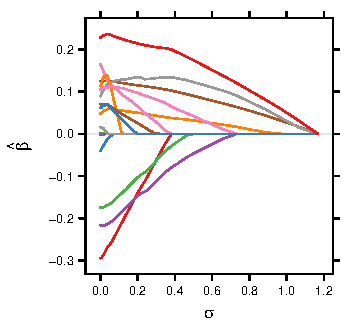
\includegraphics[]{figures/path.pdf}
% \end{column}
% \end{columns}
% \end{frame}

\begin{frame}{Predictor screening rules}
\begin{block}{motivation}
many of the solutions, \(\hat\beta\), 
along the regularization path will be \alert{sparse}, which means some 
predictors (columns) in \(X\) will be \alert{inactive}, especially
if \(p \gg n\)\medskip
\end{block}
\pause
\begin{block}{basic idea}
what if we could, based on a relatively \alert{cheap} test, determine which
predictors will be inactive before fitting the model?
\end{block}
\pause
\begin{block}{it turns out we can!}
\begin{description}
\item[safe rules] certifies that discarded predictors are not in model
\item[heuristic rules] may incorrectly discard some predictors,
                       which means problem must
                       sometimes be solved several times (in practice never more
                       than twice)
\end{description}
\end{block}
\end{frame}

\begin{frame}{Motivation for lasso strong rule}
Assume we are solving the lasso, i.e. minimizing \[g(\beta) + h(\beta), \qquad h(\beta) \coloneqq \lambda \sum_{i=1}^p |\beta_i|.\]
KKT stationarity condition is \[\boldsymbol{0} \in \nabla g(\hat\beta) + \partial h(\hat\beta),\] where
\(\partial h(\hat\beta)\) is the subdifferential for the \(\ell_1\) norm with elements
given by
\[
\partial h(\hat\beta)_i = 
\begin{cases} 
    \sign(\hat\beta_i)\lambda     & \hat\beta_i \neq 0\\ 
    [-\lambda, \lambda]           & \hat\beta_i = 0,
\end{cases}
\]
which means that \(\lvert \nabla g(\hat\beta)_i\rvert < \lambda \implies \hat\beta_i = 0\).
\end{frame}

\begin{frame}{Gradient estimate}
Assume that we are fitting a regularization \alert{path} and have
\(\hat\beta(\lambda^{(k-1)})\)---the solution for \(\lambda^{(k-1)}\)---and want
to discard predictors corresponding to the problem for \(\lambda^{(k)}\).\medskip

Basic idea: replace \(\nabla g(\hat\beta)\) with an estimate and apply the
KKT stationarity criterion, discarding predictors that are estimated to be zero.\medskip

What estimate should we use?\medskip
\end{frame}

\begin{frame}{The unit slope bound}
A simple (and conservative) estimate turns out to be \(\lambda^{(k-1)} - \lambda^{(k)}\),
i.e. assume that the gradient is piece-wise linear function with slope bounded by 1.

\centering
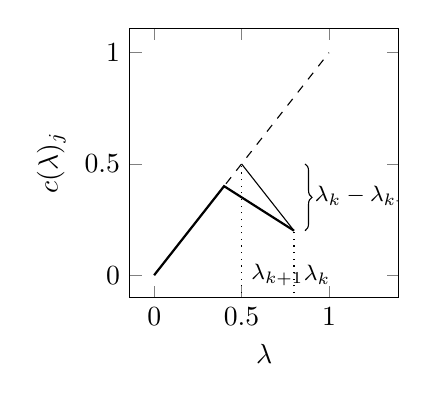
\begin{tikzpicture}
\begin{axis}[
    ylabel = \(c (\lambda)_j\),
    xlabel = \(\lambda\),
    xmax = 1.4,
    ymin = -0.1,
    width = 5cm,
    height = 5cm
]
\addplot[style = dashed]
    coordinates {
        (0,0)
        (1,1)
    };
\addplot[]
    coordinates {
        (0.8,0.2)
        (0.5,0.5)
    };
\addplot[thick]
    coordinates {
        (0.8,0.2)
        (0.4,0.4)
        (0,0)
    };
\draw [decorate,decoration={brace},xshift=4pt]
(0.8,0.5) -- (0.8,0.2)node [right,black,midway] {\footnotesize
$\lambda_{k}-\lambda_{k + 1}$};

\addplot[style=dotted]
    coordinates {
        (0.5,-0.2)
        (0.5,0.5)
    };
\addplot[style=dotted]
    coordinates {
        (0.8,-0.2)
        (0.8,0.2)
    };
\node [right] at (0.5,0) {\footnotesize$\lambda_{k + 1}$};
\node [right] at (0.8,0) {\footnotesize$\lambda_{k}$};
\end{axis}
\end{tikzpicture}

\end{frame}

\begin{frame}{The strong rule for the lasso}
Discard the \(j\)th predictor if
\[
\begin{gathered}
\underbrace{\underbrace{\left| \nabla g\left(\hat\beta(\lambda^{(k-1)})\right) \right|}_\text{previous gradient} + \underbrace{\lambda^{(k-1)} - \lambda^{(k)}}_\text{unit slope bound}}_\text{gradient prediction for \(k\)} < \lambda^{(k)}\\
\iff\\
\left| \nabla g\left(\hat\beta(\lambda^{(k-1)})\right) \right| < 2\lambda^{(k)} - \lambda^{(k-1)}
\end{gathered}
\]

Empirical results show that the strong rule leads to remarkable
performance improvements in \(p \gg n\) regime (and no penalty otherwise)~\autocite{tibshirani2012}.

\end{frame}

\begin{frame}[fragile]{Strong rule for lasso in action}
\begin{figure}
    \centering
    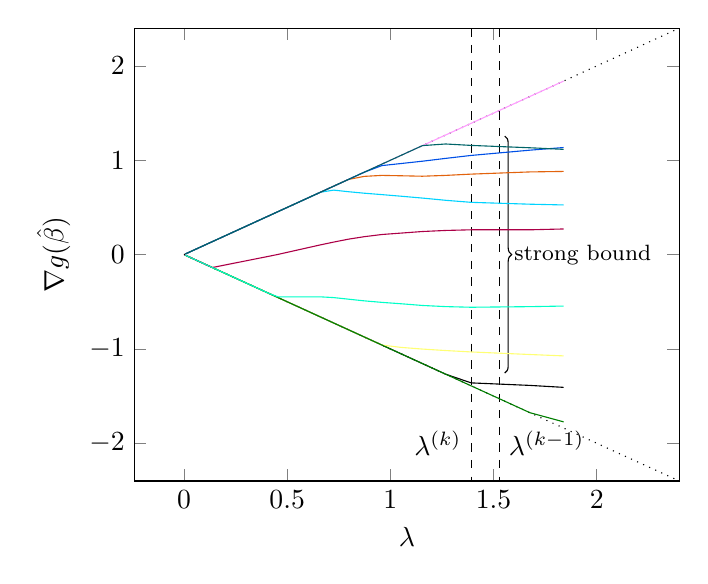
\begin{tikzpicture}
\begin{axis}[xlabel={$\lambda$}, ylabel={$\nabla g(\hat\beta)$}, width={8.5cm}, ymax={2.4}, ymin={-2.4}, xmax={2.4}]
    \draw[dashed] ({axis cs:1.3917299769873681,0}|-{rel axis cs:0,1}) -- ({axis cs:1.3917299769873681,0}|-{rel axis cs:0,0});
    \draw[dashed] ({axis cs:1.527421931643316,0}|-{rel axis cs:0,1}) -- ({axis cs:1.527421931643316,0}|-{rel axis cs:0,0});
    \addplot[dotted]
        coordinates {
            (0,0)
            (4,4)
        }
        ;
    \addplot[dotted]
        coordinates {
            (0,0)
            (4,-4)
        }
        ;
    \node 
    [left]  at 
    (1.3917299769873681,-2)
    {$\lambda^{(k)}$};
    \node 
    [right]  at 
    (1.527421931643316,-2)
    {$\lambda^{(k-1)}$};
    \draw 
    [decorate, decoration={brace}, xshift=2pt] (1.527421931643316,1.2560380223314203)
    --
    (1.527421931643316,-1.2560380223314203)
    node [right,black,midway]{\footnotesize strong bound};]
    \addplot[color={rgb,1:red,0.0;green,0.0;blue,0.0}]
        table[row sep={\\}]
        {
            \\
            1.839785124133282  -1.4077202655506813  \\
            1.6763436843655586  -1.3869613211255392  \\
            1.527421931643316  -1.372974372747998  \\
            1.3917299769873681  -1.3602300019385394  \\
            1.268092521600357  -1.2680981590214144  \\
            1.1554386769908218  -1.155442990391262  \\
            1.0527926894493917  -1.0527950409055304  \\
            0.959265488536946  -0.9592563022504802  \\
            0.8740469863817951  -0.8740136245098727  \\
            0.796399061086074  -0.7963927481850348  \\
            0.7256491634669751  -0.7256503839758264  \\
            0.6611844917574681  -0.6612256935118651  \\
            0.6024466838105537  -0.6024557616294893  \\
            0.5489269808334608  -0.5489352473825738  \\
            0.5001618207623705  -0.5001693529404507  \\
            0.4557288231095828  -0.45573568614972415  \\
            0.4152431305057957  -0.4152556144961029  \\
            0.3783540752496846  -0.37836661263540705  \\
            0.34474214199202985  -0.3447535650486027  \\
            0.31411620024661524  -0.3141266085104193  \\
            0.28621098275723084  -0.2862204663795648  \\
            0.26078478787960124  -0.26083262949872155  \\
            0.2376173860773707  -0.23766098662087795  \\
            0.21650811239921539  -0.2165478395648333  \\
            0.19727412841503122  -0.19731032632873968  \\
            0.1797488385569208  -0.17978182074774082  \\
            0.16378044714808207  -0.16381049929197253  \\
            0.1492306436212737  -0.14925802601552787  \\
            0.13597340453884807  -0.13597917728258543  \\
            0.1238939020380232  -0.12390014056372889  \\
            0.11288750924686765  -0.1128931543493642  \\
            0.1028588940563887  -0.10286403758075523  \\
            0.09372119339941025  -0.09372587998707005  \\
            0.08539526088423945  -0.08539953112836769  \\
            0.07780898126648483  -0.07781287215389417  \\
            0.07089664582130879  -0.07090019105300449  \\
            0.06459838320588741  -0.06460161348897028  \\
            0.058859640882480906  -0.05886258419611779  \\
            0.05363071261044923  -0.05363339444821467  \\
            0.04886630791457465  -0.048868751505264686  \\
            0.044525159800631986  -0.044527386309459856  \\
            0.040569667320426425  -0.040571696032346366  \\
            0.03696556989036824  -0.036967418377112635  \\
            0.033681650542687666  -0.03368333481496441  \\
            0.030689465538994057  -0.03069100018516373  \\
            0.027963098004221153  -0.027986104494638068  \\
            0.02547893344705368  -0.025499746436454043  \\
            0.023215455222500556  -0.02323441457472633  \\
            0.021153058165009335  -0.021170333145097392  \\
            0.01927387877790116  -0.01928961909526972  \\
            0.01756164050830826  -0.017575982499248043  \\
            0.016001512767459578  -0.016014580655451995  \\
            0.014579982475215659  -0.014591889448055664  \\
            0.013284737016233032  -0.01329558620642299  \\
            0.01210455759398035  -0.012114442972015223  \\
            0.011029222058889811  -0.011038229247185241  \\
            0.010049416368987792  -0.01005762338350017  \\
            0.009156653916119027  -0.00916413184208162  \\
            0.0083432020190067  -0.008350015626636686  \\
            0.00760201494646646  -0.007608223251973829  \\
            0.006926672890653523  -0.006967160900731626  \\
        }
        ;
    \addplot[color={rgb,1:red,1.0;green,1.0;blue,0.4549}]
        table[row sep={\\}]
        {
            \\
            1.839785124133282  -1.0740166024012727  \\
            1.6763436843655586  -1.0594544869154927  \\
            1.527421931643316  -1.0451902642046422  \\
            1.3917299769873681  -1.0321932427787441  \\
            1.268092521600357  -1.0173512166391305  \\
            1.1554386769908218  -1.0016060767090929  \\
            1.0527926894493917  -0.9841837507773538  \\
            0.959265488536946  -0.9592622167171292  \\
            0.8740469863817951  -0.8740301158898205  \\
            0.796399061086074  -0.7963925883654892  \\
            0.7256491634669751  -0.7256482826596983  \\
            0.6611844917574681  -0.6612071636572264  \\
            0.6024466838105537  -0.6024283924821208  \\
            0.5489269808334608  -0.5489102878041107  \\
            0.5001618207623705  -0.5001466106971787  \\
            0.4557288231095828  -0.4557149642646659  \\
            0.4152431305057957  -0.4152434412422857  \\
            0.3783540752496846  -0.37835507617537856  \\
            0.34474214199202985  -0.3447430538877129  \\
            0.31411620024661524  -0.3141170311319773  \\
            0.28621098275723084  -0.28621173982902726  \\
            0.26078478787960124  -0.26077574467382625  \\
            0.2376173860773707  -0.23760916619742814  \\
            0.21650811239921539  -0.2165006227546474  \\
            0.19727412841503122  -0.1972673041298264  \\
            0.1797488385569208  -0.17974262052240483  \\
            0.16378044714808207  -0.16377478150661473  \\
            0.1492306436212737  -0.1492254812997791  \\
            0.13597340453884807  -0.1359712745522819  \\
            0.1238939020380232  -0.12387127117967824  \\
            0.11288750924686765  -0.11286684252948499  \\
            0.1028588940563887  -0.10284006317743971  \\
            0.09372119339941025  -0.09370403540352074  \\
            0.08539526088423945  -0.0853796271574143  \\
            0.07780898126648483  -0.07779473639686238  \\
            0.07089664582130879  -0.07088366642664293  \\
            0.06459838320588741  -0.064586556864871  \\
            0.058859640882480906  -0.058848865161005286  \\
            0.05363071261044923  -0.05362089417437037  \\
            0.04886630791457465  -0.048857361721296184  \\
            0.044525159800631986  -0.04451700836250741  \\
            0.040569667320426425  -0.04056224003359853  \\
            0.03696556989036824  -0.03695880242323147  \\
            0.033681650542687666  -0.033675484278679314  \\
            0.030689465538994057  -0.03068384706888505  \\
            0.027963098004221153  -0.027940863534424515  \\
            0.02547893344705368  -0.025458479653743024  \\
            0.023215455222500556  -0.02319681458390611  \\
            0.021153058165009335  -0.02113607343979051  \\
            0.01927387877790116  -0.019258402927784055  \\
            0.01756164050830826  -0.01754753949004626  \\
            0.016001512767459578  -0.015988664444795693  \\
            0.014579982475215659  -0.0145682755621255  \\
            0.013284737016233032  -0.013274070113036017  \\
            0.01210455759398035  -0.012094838309064118  \\
            0.011029222058889811  -0.01102036620845793  \\
            0.010049416368987792  -0.010041347247900375  \\
            0.009156653916119027  -0.00914930163350964  \\
            0.0083432020190067  -0.008336502892920351  \\
            0.00760201494646646  -0.007595910952278082  \\
            0.006926672890653523  -0.0069078250525788755  \\
        }
        ;
    \addplot[color={rgb,1:red,1.0;green,0.6078;blue,1.0}]
        table[row sep={\\}]
        {
            \\
            1.839785124133282  1.8397851241332814  \\
            1.6763436843655586  1.6763435737142731  \\
            1.527421931643316  1.5274217418527607  \\
            1.3917299769873681  1.391729804057265  \\
            1.268092521600357  1.2680914205021188  \\
            1.1554386769908218  1.1554371367955463  \\
            1.0527926894493917  1.0527919387552134  \\
            0.959265488536946  0.9592702558864394  \\
            0.8740469863817951  0.8740672706735734  \\
            0.796399061086074  0.7964046343401125  \\
            0.7256491634669751  0.7256483944132225  \\
            0.6611844917574681  0.6611605169065458  \\
            0.6024466838105537  0.6024664616368461  \\
            0.5489269808334608  0.5489449997288162  \\
            0.5001618207623705  0.5001782389043823  \\
            0.4557288231095828  0.4557437827091072  \\
            0.4152431305057957  0.4152372733166853  \\
            0.3783540752496846  0.37834810595204593  \\
            0.34474214199202985  0.34473670330304995  \\
            0.31411620024661524  0.31411124471572427  \\
            0.28621098275723084  0.2862064674620465  \\
            0.26078478787960124  0.26077418627403975  \\
            0.2376173860773707  0.2376077130814579  \\
            0.21650811239921539  0.21649929873953025  \\
            0.19727412841503122  0.19726609773659273  \\
            0.1797488385569208  0.17974152130182128  \\
            0.16378044714808207  0.16377377993775838  \\
            0.1492306436212737  0.14922456870753986  \\
            0.13597340453884807  0.1359975805661932  \\
            0.1238939020380232  0.12395417963980454  \\
            0.11288750924686765  0.11294254102291855  \\
            0.1028588940563887  0.10290903723355237  \\
            0.09372119339941025  0.09376688199557048  \\
            0.08539526088423945  0.08543689063144173  \\
            0.07780898126648483  0.07784691274168168  \\
            0.07089664582130879  0.07093120756879294  \\
            0.06459838320588741  0.06462987458298106  \\
            0.058859640882480906  0.05888833465242757  \\
            0.05363071261044923  0.05365685730495745  \\
            0.04886630791457465  0.04889012998648044  \\
            0.044525159800631986  0.044546865585326216  \\
            0.040569667320426425  0.040589444823032055  \\
            0.03696556989036824  0.0369835904141515  \\
            0.033681650542687666  0.033698070172804774  \\
            0.030689465538994057  0.030704426494426045  \\
            0.027963098004221153  0.02802531416566563  \\
            0.02547893344705368  0.0255363416101223  \\
            0.023215455222500556  0.02326777514724212  \\
            0.021153058165009335  0.021200730310042087  \\
            0.01927387877790116  0.01931731586357297  \\
            0.01756164050830826  0.01760121876304457  \\
            0.016001512767459578  0.01603757499912812  \\
            0.014579982475215659  0.014612841037614432  \\
            0.013284737016233032  0.013314676514510375  \\
            0.01210455759398035  0.012131837349747548  \\
            0.011029222058889811  0.011054078356340695  \\
            0.010049416368987792  0.010072064501480335  \\
            0.009156653916119027  0.009177290050941603  \\
            0.0083432020190067  0.008362004896487108  \\
            0.00760201494646646  0.007619147428134818  \\
            0.006926672890653523  0.006991613998442512  \\
        }
        ;
    \addplot[color={rgb,1:red,0.0;green,0.8275;blue,1.0}]
        table[row sep={\\}]
        {
            \\
            1.839785124133282  0.5262818345203535  \\
            1.6763436843655586  0.534233758654948  \\
            1.527421931643316  0.5445507732951834  \\
            1.3917299769873681  0.5539512511560487  \\
            1.268092521600357  0.5755617465578776  \\
            1.1554386769908218  0.5991746832820806  \\
            1.0527926894493917  0.618744458910842  \\
            0.959265488536946  0.6357746362395237  \\
            0.8740469863817951  0.6507163288487767  \\
            0.796399061086074  0.6667630765307442  \\
            0.7256491634669751  0.6834952403873034  \\
            0.6611844917574681  0.6611968292640323  \\
            0.6024466838105537  0.6024363329713686  \\
            0.5489269808334608  0.5489175474749682  \\
            0.5001618207623705  0.5001532254393263  \\
            0.4557288231095828  0.4557209913713487  \\
            0.4152431305057957  0.4152443377154589  \\
            0.3783540752496846  0.37835416163470703  \\
            0.34474214199202985  0.34474222067869875  \\
            0.31411620024661524  0.3141162719429976  \\
            0.28621098275723084  0.2862110480843047  \\
            0.26078478787960124  0.2607872837299235  \\
            0.2376173860773707  0.23761965606434202  \\
            0.21650811239921539  0.216510180722962  \\
            0.19727412841503122  0.1972760129945995  \\
            0.1797488385569208  0.17975055571563442  \\
            0.16378044714808207  0.1637820117591483  \\
            0.1492306436212737  0.14923206923660504  \\
            0.13597340453884807  0.13596883260158948  \\
            0.1238939020380232  0.12387996029846464  \\
            0.11288750924686765  0.11287478604400487  \\
            0.1028588940563887  0.10284730110868157  \\
            0.09372119339941025  0.09371063033712901  \\
            0.08539526088423945  0.08538563621529799  \\
            0.07780898126648483  0.07780021162660539  \\
            0.07089664582130879  0.07088865525206595  \\
            0.06459838320588741  0.0645911024967932  \\
            0.058859640882480906  0.05885300697151626  \\
            0.05363071261044923  0.053624668037850896  \\
            0.04886630791457465  0.04886080032514656  \\
            0.044525159800631986  0.044520141490269005  \\
            0.040569667320426425  0.04056509482292512  \\
            0.03696556989036824  0.03696140360094269  \\
            0.033681650542687666  0.033677854374931836  \\
            0.030689465538994057  0.03068600661231927  \\
            0.027963098004221153  0.02795465341355136  \\
            0.02547893344705368  0.02547105016933694  \\
            0.023215455222500556  0.023208269620523928  \\
            0.021153058165009335  0.02114651087569309  \\
            0.01927387877790116  0.01926791313120384  \\
            0.01756164050830826  0.017556204833213837  \\
            0.016001512767459578  0.015996559982759187  \\
            0.014579982475215659  0.014575469682257702  \\
            0.013284737016233032  0.013280625127363797  \\
            0.01210455759398035  0.01210081099398526  \\
            0.011029222058889811  0.011025808296512346  \\
            0.010049416368987792  0.010046305875851416  \\
            0.009156653916119027  0.009153819750619857  \\
            0.0083432020190067  0.008340619632959163  \\
            0.00760201494646646  0.007599661972478075  \\
            0.006926672890653523  0.006938247028719643  \\
        }
        ;
    \addplot[color={rgb,1:red,0.8863;green,0.3882;blue,0.051}]
        table[row sep={\\}]
        {
            \\
            1.839785124133282  0.8817437504727766  \\
            1.6763436843655586  0.8764029656563675  \\
            1.527421931643316  0.8642526181103705  \\
            1.3917299769873681  0.8531816704687174  \\
            1.268092521600357  0.8396096892176024  \\
            1.1554386769908218  0.8308134826424433  \\
            1.0527926894493917  0.8356460692390775  \\
            0.959265488536946  0.8395549699310465  \\
            0.8740469863817951  0.8294534875626539  \\
            0.796399061086074  0.7964048236049572  \\
            0.7256491634669751  0.7256489759532192  \\
            0.6611844917574681  0.6611630441550489  \\
            0.6024466838105537  0.6024671125855324  \\
            0.5489269808334608  0.5489455962588012  \\
            0.5001618207623705  0.500178782441049  \\
            0.4557288231095828  0.4557442779594743  \\
            0.4152431305057957  0.4152387874408213  \\
            0.3783540752496846  0.37835037867040106  \\
            0.34474214199202985  0.34473877402041775  \\
            0.31411620024661524  0.31411313147627523  \\
            0.28621098275723084  0.2862081866079899  \\
            0.26078478787960124  0.2607783531703273  \\
            0.2376173860773707  0.23761151617256815  \\
            0.21650811239921539  0.21650276397148918  \\
            0.19727412841503122  0.19726925512689003  \\
            0.1797488385569208  0.17974439819826646  \\
            0.16378044714808207  0.16377640125865256  \\
            0.1492306436212737  0.1492269571575102  \\
            0.13597340453884807  0.13599652652692876  \\
            0.1238939020380232  0.12395464551935445  \\
            0.11288750924686765  0.11294296080154165  \\
            0.1028588940563887  0.10290941970627922  \\
            0.09372119339941025  0.09376723049044494  \\
            0.08539526088423945  0.08543720816699153  \\
            0.07780898126648483  0.0778472020682489  \\
            0.07089664582130879  0.07093147119238505  \\
            0.06459838320588741  0.06463011478698018  \\
            0.058859640882480906  0.05888855351736519  \\
            0.05363071261044923  0.05365705672653711  \\
            0.04886630791457465  0.04889031169199658  \\
            0.044525159800631986  0.04454703114862497  \\
            0.040569667320426425  0.04058959567814366  \\
            0.03696556989036824  0.036983727867710724  \\
            0.033681650542687666  0.03369819541536849  \\
            0.030689465538994057  0.03070454061078536  \\
            0.027963098004221153  0.028023191776597366  \\
            0.02547893344705368  0.025534398359090122  \\
            0.023215455222500556  0.023266003958779074  \\
            0.021153058165009335  0.021199116458854465  \\
            0.01927387877790116  0.01931584538232567  \\
            0.01756164050830826  0.017599878915296418  \\
            0.016001512767459578  0.016036354179760792  \\
            0.014579982475215659  0.014611728672475106  \\
            0.013284737016233032  0.013313662968824183  \\
            0.01210455759398035  0.012130913844666491  \\
            0.011029222058889811  0.011053236892905912  \\
            0.010049416368987792  0.010071297791337593  \\
            0.009156653916119027  0.009176591453214976  \\
            0.0083432020190067  0.008361368360257462  \\
            0.00760201494646646  0.007618567440028876  \\
            0.006926672890653523  0.0069786583100767885  \\
        }
        ;
    \addplot[color={rgb,1:red,0.0;green,0.4941;blue,0.0}]
        table[row sep={\\}]
        {
            \\
            1.839785124133282  -1.7735789352411289  \\
            1.6763436843655586  -1.6763436843655581  \\
            1.527421931643316  -1.5274219316433155  \\
            1.3917299769873681  -1.391729976987368  \\
            1.268092521600357  -1.2680925216003567  \\
            1.1554386769908218  -1.1554387352256574  \\
            1.0527926894493917  -1.0527927253180733  \\
            0.959265488536946  -0.9592654218675132  \\
            0.8740469863817951  -0.8740488675653486  \\
            0.796399061086074  -0.796401157977832  \\
            0.7256491634669751  -0.7256498327295953  \\
            0.6611844917574681  -0.6611797549521219  \\
            0.6024466838105537  -0.602454516052506  \\
            0.5489269808334608  -0.5489341243907603  \\
            0.5001618207623705  -0.5001683297055934  \\
            0.4557288231095828  -0.45573475381622813  \\
            0.4152431305057957  -0.41524297572645497  \\
            0.3783540752496846  -0.3783537279901447  \\
            0.34474214199202985  -0.3447418256244353  \\
            0.31411620024661524  -0.3141159119842545  \\
            0.28621098275723084  -0.28621072010330356  \\
            0.26078478787960124  -0.26078846836502  \\
            0.2376173860773707  -0.23762073189963928  \\
            0.21650811239921539  -0.21651116098615403  \\
            0.19727412841503122  -0.19727690617391602  \\
            0.1797488385569208  -0.1797513695473617  \\
            0.16378044714808207  -0.16378275329230824  \\
            0.1492306436212737  -0.1492327448940026  \\
            0.13597340453884807  -0.1359688467753483  \\
            0.1238939020380232  -0.12388826866245196  \\
            0.11288750924686765  -0.11288236943386355  \\
            0.1028588940563887  -0.10285421083493197  \\
            0.09372119339941025  -0.09371692622240055  \\
            0.08539526088423945  -0.0853913727914745  \\
            0.07780898126648483  -0.07780543858116488  \\
            0.07089664582130879  -0.07089341785838886  \\
            0.06459838320588741  -0.06459544200629642  \\
            0.058859640882480906  -0.05885696097095554  \\
            0.05363071261044923  -0.05362827077487783  \\
            0.04886630791457465  -0.04886408300494525  \\
            0.044525159800631986  -0.04452313254584203  \\
            0.040569667320426425  -0.0405678201613648  \\
            0.03696556989036824  -0.036963886827826836  \\
            0.033681650542687666  -0.03368011699878376  \\
            0.030689465538994057  -0.030688068230903993  \\
            0.027963098004221153  -0.02795481245972661  \\
            0.02547893344705368  -0.02547131917080111  \\
            0.023215455222500556  -0.023208516846951927  \\
            0.021153058165009335  -0.021146736171030956  \\
            0.01927387877790116  -0.019268118412388815  \\
            0.01756164050830826  -0.017556391877790754  \\
            0.016001512767459578  -0.015996730410811653  \\
            0.014579982475215659  -0.014575624969951538  \\
            0.013284737016233032  -0.013280766619727026  \\
            0.01210455759398035  -0.012100939916557136  \\
            0.011029222058889811  -0.011025925765957846  \\
            0.010049416368987792  -0.010046412909635379  \\
            0.009156653916119027  -0.009153917275817458  \\
            0.0083432020190067  -0.008340708494287197  \\
            0.00760201494646646  -0.007599742939610854  \\
            0.006926672890653523  -0.006909246075506272  \\
        }
        ;
    \addplot[color={rgb,1:red,0.0;green,0.3137;blue,0.902}]
        table[row sep={\\}]
        {
            \\
            1.839785124133282  1.135089754174434  \\
            1.6763436843655586  1.1071139623655615  \\
            1.527421931643316  1.0779239477935385  \\
            1.3917299769873681  1.051327105647608  \\
            1.268092521600357  1.0200279843113864  \\
            1.1554386769908218  0.9900664325473005  \\
            1.0527926894493917  0.9656388790664223  \\
            0.959265488536946  0.9437444131949158  \\
            0.8740469863817951  0.8740485689218533  \\
            0.796399061086074  0.7963995354471453  \\
            0.7256491634669751  0.7256491217992942  \\
            0.6611844917574681  0.6611835673153322  \\
            0.6024466838105537  0.6024491755659228  \\
            0.5489269808334608  0.5489292509956886  \\
            0.5001618207623705  0.5001638892494293  \\
            0.4557288231095828  0.455730707837952  \\
            0.4152431305057957  0.41524492767887466  \\
            0.3783540752496846  0.37835699281762414  \\
            0.34474214199202985  0.3447448002387928  \\
            0.31411620024661524  0.31411862234205856  \\
            0.28621098275723084  0.28621318968039045  \\
            0.26078478787960124  0.26078947152604376  \\
            0.2376173860773707  0.2376216655364002  \\
            0.21650811239921539  0.21651201168186554  \\
            0.19727412841503122  0.19727768129614762  \\
            0.1797488385569208  0.17975207580987074  \\
            0.16378044714808207  0.16378339681240223  \\
            0.1492306436212737  0.1492333312455451  \\
            0.13597340453884807  0.13598458950805786  \\
            0.1238939020380232  0.12391877366999463  \\
            0.11288750924686765  0.11291019881807988  \\
            0.1028588940563887  0.1028795680134583  \\
            0.09372119339941025  0.09374003073928097  \\
            0.08539526088423945  0.0854124247667541  \\
            0.07780898126648483  0.07782462035698239  \\
            0.07089664582130879  0.07091089557810949  \\
            0.06459838320588741  0.06461136705356804  \\
            0.058859640882480906  0.05887147128091845  \\
            0.05363071261044923  0.05364149202889543  \\
            0.04886630791457465  0.04887612971919543  \\
            0.044525159800631986  0.04453410906320032  \\
            0.040569667320426425  0.04057782155517334  \\
            0.03696556989036824  0.03697299972537414  \\
            0.033681650542687666  0.033688420331629006  \\
            0.030689465538994057  0.030695633918544067  \\
            0.027963098004221153  0.02798984504654397  \\
            0.02547893344705368  0.02550355258227658  \\
            0.023215455222500556  0.023237889904029186  \\
            0.021153058165009335  0.02117349984475035  \\
            0.01927387877790116  0.019292504475629687  \\
            0.01756164050830826  0.017578611550392052  \\
            0.016001512767459578  0.01601697614893885  \\
            0.014579982475215659  0.014594072132502944  \\
            0.013284737016233032  0.013297574987199634  \\
            0.01210455759398035  0.012116255074989191  \\
            0.011029222058889811  0.011039880367925416  \\
            0.010049416368987792  0.01005912782322409  \\
            0.009156653916119027  0.009165502631526783  \\
            0.0083432020190067  0.008351264638925694  \\
            0.00760201494646646  0.007609361305453279  \\
            0.006926672890653523  0.006948687748096627  \\
        }
        ;
    \addplot[color={rgb,1:red,0.6745;green,0.0;blue,0.2784}]
        table[row sep={\\}]
        {
            \\
            1.839785124133282  0.27166717270336277  \\
            1.6763436843655586  0.26282311169114886  \\
            1.527421931643316  0.26284489047542386  \\
            1.3917299769873681  0.2628647463964542  \\
            1.268092521600357  0.2558751900981948  \\
            1.1554386769908218  0.24463973790676177  \\
            1.0527926894493917  0.2280796660946305  \\
            0.959265488536946  0.21294150755378927  \\
            0.8740469863817951  0.18996460284401231  \\
            0.796399061086074  0.16333980815528096  \\
            0.7256491634669751  0.13272353146394295  \\
            0.6611844917574681  0.10302551991449099  \\
            0.6024466838105537  0.07413244085917409  \\
            0.5489269808334608  0.04779948346551989  \\
            0.5001618207623705  0.023805875011035642  \\
            0.4557288231095828  0.001943792602986445  \\
            0.4152431305057957  -0.01610576196058167  \\
            0.3783540752496846  -0.03217249429607616  \\
            0.34474214199202985  -0.04681218681148503  \\
            0.31411620024661524  -0.06015132938878707  \\
            0.28621098275723084  -0.07230545930373283  \\
            0.26078478787960124  -0.08337787969527607  \\
            0.2376173860773707  -0.09346862584109146  \\
            0.21650811239921539  -0.10266293896436345  \\
            0.19727412841503122  -0.11104045465152161  \\
            0.1797488385569208  -0.11867373493443248  \\
            0.16378044714808207  -0.1256288956352116  \\
            0.1492306436212737  -0.1319661790285596  \\
            0.13597340453884807  -0.13597721900505028  \\
            0.1238939020380232  -0.12390210787111552  \\
            0.11288750924686765  -0.1128949956999519  \\
            0.1028588940563887  -0.10286571545449083  \\
            0.09372119339941025  -0.09372740880335872  \\
            0.08539526088423945  -0.08540092412883162  \\
            0.07780898126648483  -0.077814141404036  \\
            0.07089664582130879  -0.07090134754646193  \\
            0.06459838320588741  -0.06460266724273649  \\
            0.058859640882480906  -0.05886354433730366  \\
            0.05363071261044923  -0.05363426929310386  \\
            0.04886630791457465  -0.04886954863134488  \\
            0.044525159800631986  -0.044528112621056194  \\
            0.040569667320426425  -0.04057235782042237  \\
            0.03696556989036824  -0.036968021373760054  \\
            0.033681650542687666  -0.0336838842430515  \\
            0.030689465538994057  -0.030691500803573968  \\
            0.027963098004221153  -0.02797089594992417  \\
            0.02547893344705368  -0.025486130402715287  \\
            0.023215455222500556  -0.02322201391048899  \\
            0.021153058165009335  -0.02115903421129019  \\
            0.01927387877790116  -0.019279323928899236  \\
            0.01756164050830826  -0.017566601927102063  \\
            0.016001512767459578  -0.016006033427482063  \\
            0.014579982475215659  -0.014584101532261178  \\
            0.013284737016233032  -0.013288490147603306  \\
            0.01210455759398035  -0.012107977307503735  \\
            0.011029222058889811  -0.011032337974488993  \\
            0.010049416368987792  -0.010052255475232856  \\
            0.009156653916119027  -0.009159240803990283  \\
            0.0083432020190067  -0.008345559094889304  \\
            0.00760201494646646  -0.00760416262622404  \\
            0.006926672890653523  -0.006930576992560517  \\
        }
        ;
    \addplot[color={rgb,1:red,0.0;green,1.0;blue,0.7843}]
        table[row sep={\\}]
        {
            \\
            1.839785124133282  -0.5457122136864775  \\
            1.6763436843655586  -0.5519040341475189  \\
            1.527421931643316  -0.5552602552360572  \\
            1.3917299769873681  -0.5583183135173444  \\
            1.268092521600357  -0.551557927335853  \\
            1.1554386769908218  -0.5394217331984487  \\
            1.0527926894493917  -0.5214957209340106  \\
            0.959265488536946  -0.5066338186587006  \\
            0.8740469863817951  -0.4906790683791963  \\
            0.796399061086074  -0.47262329580902657  \\
            0.7256491634669751  -0.45594919886022495  \\
            0.6611844917574681  -0.44797798297355074  \\
            0.6024466838105537  -0.44810656671413673  \\
            0.5489269808334608  -0.4482192285223354  \\
            0.5001618207623705  -0.4483218778597154  \\
            0.4557288231095828  -0.4484154081125965  \\
            0.4152431305057957  -0.4152433406358467  \\
            0.3783540752496846  -0.3783537243458599  \\
            0.34474214199202985  -0.3447418222699672  \\
            0.31411620024661524  -0.31411590892779007  \\
            0.28621098275723084  -0.28621071731836717  \\
            0.26078478787960124  -0.2607844443394749  \\
            0.2376173860773707  -0.23761706965357263  \\
            0.21650811239921539  -0.2165078240838153  \\
            0.19727412841503122  -0.19727386571277947  \\
            0.1797488385569208  -0.17974859919241318  \\
            0.16378044714808207  -0.16378022904805767  \\
            0.1492306436212737  -0.14923044489665452  \\
            0.13597340453884807  -0.13596704132892784  \\
            0.1238939020380232  -0.12387984433101144  \\
            0.11288750924686765  -0.11287468245352944  \\
            0.1028588940563887  -0.10284720672005845  \\
            0.09372119339941025  -0.0937105443337278  \\
            0.08539526088423945  -0.08538555785220199  \\
            0.07780898126648483  -0.07780014022507103  \\
            0.07089664582130879  -0.07088859019364735  \\
            0.06459838320588741  -0.06459104321798524  \\
            0.058859640882480906  -0.05885295295887438  \\
            0.05363071261044923  -0.053624618823543226  \\
            0.04886630791457465  -0.04886075548290233  \\
            0.044525159800631986  -0.04452010063168643  \\
            0.040569667320426425  -0.0405650575941064  \\
            0.03696556989036824  -0.036961369679429854  \\
            0.033681650542687666  -0.03367782346691275  \\
            0.030689465538994057  -0.030685978450083095  \\
            0.027963098004221153  -0.027949930887841427  \\
            0.02547893344705368  -0.025466775773739327  \\
            0.023215455222500556  -0.023204375570947157  \\
            0.021153058165009335  -0.021142962771972983  \\
            0.01927387877790116  -0.019264680231371355  \\
            0.01756164050830826  -0.017553259135294503  \\
            0.016001512767459578  -0.015993875972524253  \\
            0.014579982475215659  -0.014573024112094744  \\
            0.013284737016233032  -0.013278396814913744  \\
            0.01210455759398035  -0.012098780638671975  \\
            0.011029222058889811  -0.01102395831236918  \\
            0.010049416368987792  -0.01004462023920063  \\
            0.009156653916119027  -0.009152283861283585  \\
            0.0083432020190067  -0.008339220187798731  \\
            0.00760201494646646  -0.0075983868501685505  \\
            0.006926672890653523  -0.00691964342724483  \\
        }
        ;
    \addplot[color={rgb,1:red,0.0;green,0.3922;blue,0.4078}]
        table[row sep={\\}]
        {
            \\
            1.839785124133282  1.1157355634468402  \\
            1.6763436843655586  1.1325274950490352  \\
            1.527421931643316  1.1456001545954875  \\
            1.3917299769873681  1.157511464002459  \\
            1.268092521600357  1.1726662727727077  \\
            1.1554386769908218  1.155438676990822  \\
            1.0527926894493917  1.0527926894493917  \\
            0.959265488536946  0.9592654885369458  \\
            0.8740469863817951  0.8740469863817953  \\
            0.796399061086074  0.7963990610860745  \\
            0.7256491634669751  0.7256491634669753  \\
            0.6611844917574681  0.6611844917574682  \\
            0.6024466838105537  0.6024466838105534  \\
            0.5489269808334608  0.5489269808334606  \\
            0.5001618207623705  0.5001618207623703  \\
            0.4557288231095828  0.4557288231095826  \\
            0.4152431305057957  0.4152431305057954  \\
            0.3783540752496846  0.3783540752496847  \\
            0.34474214199202985  0.34474214199202957  \\
            0.31411620024661524  0.3141162002466153  \\
            0.28621098275723084  0.286210982757231  \\
            0.26078478787960124  0.2607847878796014  \\
            0.2376173860773707  0.2376173860773704  \\
            0.21650811239921539  0.21650811239921566  \\
            0.19727412841503122  0.1972741284150313  \\
            0.1797488385569208  0.17974883855692073  \\
            0.16378044714808207  0.16378044714808232  \\
            0.1492306436212737  0.1492306436212739  \\
            0.13597340453884807  0.13597340453884837  \\
            0.1238939020380232  0.1238939020380234  \\
            0.11288750924686765  0.11288750924686786  \\
            0.1028588940563887  0.10285889405638869  \\
            0.09372119339941025  0.0937211933994106  \\
            0.08539526088423945  0.08539526088423952  \\
            0.07780898126648483  0.07780898126648492  \\
            0.07089664582130879  0.0708966458213087  \\
            0.06459838320588741  0.06459838320588732  \\
            0.058859640882480906  0.058859640882480996  \\
            0.05363071261044923  0.053630712610449466  \\
            0.04886630791457465  0.04886630791457489  \\
            0.044525159800631986  0.044525159800631896  \\
            0.040569667320426425  0.04056966732042648  \\
            0.03696556989036824  0.036965569890368276  \\
            0.033681650542687666  0.03368165054268768  \\
            0.030689465538994057  0.03068946553899421  \\
            0.027963098004221153  0.027963098004221205  \\
            0.02547893344705368  0.025478933447053688  \\
            0.023215455222500556  0.023215455222500833  \\
            0.021153058165009335  0.021153058165009654  \\
            0.01927387877790116  0.01927387877790155  \\
            0.01756164050830826  0.017561640508308246  \\
            0.016001512767459578  0.016001512767459588  \\
            0.014579982475215659  0.014579982475215983  \\
            0.013284737016233032  0.013284737016233308  \\
            0.01210455759398035  0.012104557593980486  \\
            0.011029222058889811  0.011029222058889772  \\
            0.010049416368987792  0.01004941636898815  \\
            0.009156653916119027  0.009156653916119119  \\
            0.0083432020190067  0.00834320201900672  \\
            0.00760201494646646  0.007602014946466475  \\
            0.006926672890653523  0.006926672890653485  \\
        }
        ;
\end{axis}
\end{tikzpicture}

\end{figure}
\end{frame}

\begin{frame}{Strong rule for SLOPE}
Exactly the same idea as for lasso strong rule.\medskip

The subdifferential for SLOPE is is the
set of all \(g \in \mathbb{R}^p\) such that
\[
g_{\mathcal{A}_i} =
\left\{s \in \mathbb{R}^{\mathop{\mathrm{card}}{\mathcal{A}_i}} \bigm\vert 
\begin{cases}
  \mathop{\mathrm{cumsum}}(|s|_\downarrow - \lambda_{R(s)_{\mathcal{A}_i}}) \preceq \mathbf{0} &\text{if } \beta_{\mathcal{A}_i} = \mathbf{0},\\
  \mathop{\mathrm{cumsum}}(|s|_\downarrow - \lambda_{R(s)_{\mathcal{A}_i}}) \preceq \mathbf{0} \\\quad\,\wedge\, \sum_{j \in \mathcal{A}_i}\left(|s_j| - \lambda_{R(s)_j}\right) = 0 & \text{otherwise.}
\end{cases}
\right\}
\]
\(\mathcal{A}_i\) defines a \alert{cluster} containing indices of coefficients
equal in absolute value.\medskip

\(R(x)\) is an operator that returns the \alert{ranks} of elements in \(|x|\).\medskip

\(|x|_\downarrow\) returns the absolute values of \(x\) sorted in non-increasing
order.\medskip
\end{frame}

\begin{frame}[fragile]{Strong rule algorithm for SLOPE}
\label{alg:sparsity-rule}
\begin{algorithmic}[1]
\Require \(c \in \mathbb{R}^p\), 
         \(\lambda \in \mathbb{R}^p\), where 
         \(\lambda_1 \geq \cdots \geq \lambda_p \geq 0\).
\State \(\mathcal{S}, \mathcal{B} \gets \varnothing\)
\For{\(i \gets 1,\dots,p\)}
  \State \(\mathcal{B} \gets \mathcal{B} \cup \{i\}\)
  \If{\(\sum_{j \in \mathcal{B}}\big(c_j - \lambda_j\big) \geq 0\)}
    \State \(\mathcal{S} \gets \mathcal{S} \cup \mathcal{B}\)
    \State \(\mathcal{B} \gets \varnothing\)
  \EndIf
\EndFor
\State Return \(\mathcal{S}\)
\end{algorithmic}
\medskip
Set
\[
    c \coloneqq \lvert \nabla g(\hat\beta)+ \lambda^{(k-1)} - \lambda^{(k)}\rvert_\downarrow \qquad \lambda \coloneqq \lambda^{(k)},
\] and run the algorithm above;
the result is the predicted support for \(\hat\beta(\lambda^{(k)})\) (subject to a 
permutation).
\end{frame}

\begin{frame}{Efficiency for simulated data}
\begin{figure}
\centering
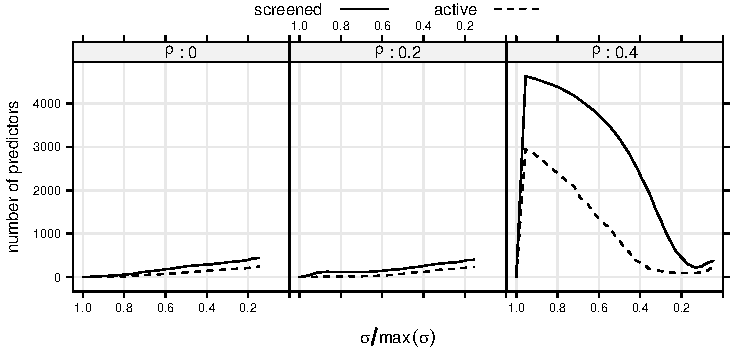
\includegraphics[width=\linewidth]{figures/gaussian.pdf}
\caption{Gaussian design, \(X \in \mathbb{R}^{200\times 5000}\),
predictors pairwise correlated with correlation \(\rho\). There were no violations of
the strong rule here.}
\end{figure}
\end{frame}

\begin{frame}{Efficiency for real data}
\begin{figure}
\centering
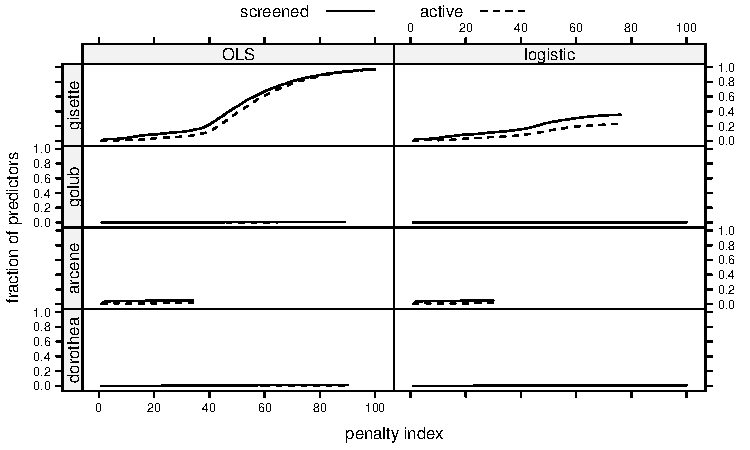
\includegraphics[width=\linewidth]{figures/efficiency-real.pdf}
\caption{Efficiency for real data sets. The dimensions of the predictor matrices
are \(100 \times 9920\) (arcene), \(800\times 88119\) (dorothea), \(6000\times 4955\)
(gisette), and \(38 \times 7129\) (golub).}
\end{figure}
\end{frame}

\begin{frame}{Violations}
Violations may occur if the unit slope bound fails, which can occur if
ordering permutation of absolute gradient changes, or any predictor becomes active between
\(\lambda^{(k-1)}\) and \(\lambda^{(k)}\).\medskip

Thankfully, such violations turn out to be \alert{rare}.
\begin{figure}
\centering
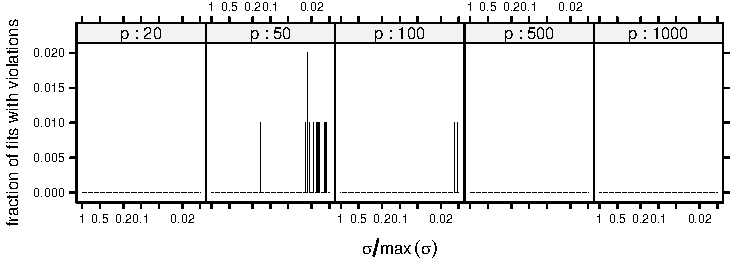
\includegraphics[width=\linewidth]{figures/violations.pdf}
\caption{Violations for sorted \(\ell_1\) regularized least squares regression
with predictors pairwise correlated with \(\rho = 0.5\). \(X\in \mathbb{R}^{100 \times p}\).}
\end{figure}
\end{frame}

\begin{frame}{Performance}
\begin{figure}
\centering
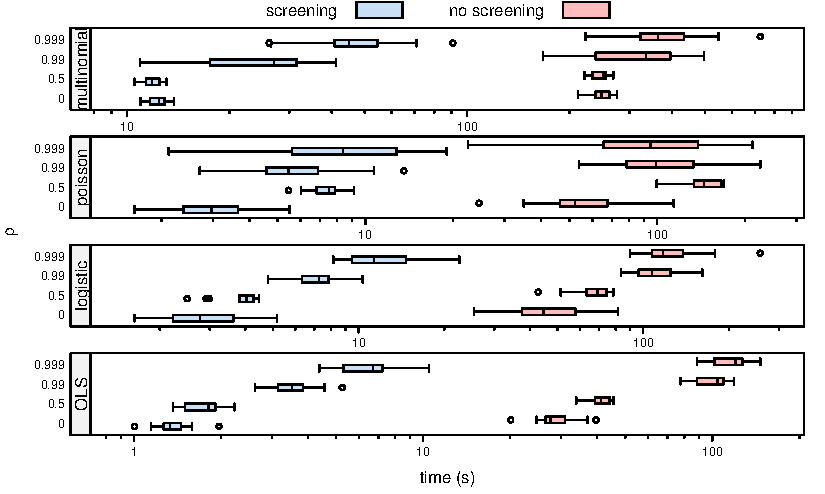
\includegraphics[width=\linewidth]{figures/performance.pdf}
\caption{Performance benchmarks for various generalized linear models
with \(X \in \mathbb{R}^{200 \times 20000}\). Predictors are autocorrelated through an
\(\operatorname{AR}(1)\) process with correlation \(\rho\).}
\end{figure}
\end{frame}

\begin{frame}{Algorithms}
The original strong rule paper~\autocite{tibshirani2012} presents two
strategies for using the screening rule.  For SLOPE, we have two \alert{slightly}
modified versions of these algorithms

\begin{block}{strong set algorithm}
initialize \(\mathcal{E}\) with strong rule set
\begin{enumerate}
    \item fit SLOPE to predictors in \(\mathcal{E}\)
    \item check KKT criteria against \(\mathcal{E}^C\); 
              if there are any failures, add predictors that
              fail the check to \(\mathcal{E}\) and go back to 1
\end{enumerate}
\end{block}
\pause
\begin{block}{previous set algorithm}
initialize \(\mathcal{E}\) with ever-active predictors
\begin{enumerate}
    \item fit SLOPE to predictors in \(\mathcal{E}\)
    \item check KKT criteria against predictors in \alert{strong} set
        \begin{itemize}
            \item if there are any failures, include these predictors in \(\mathcal{E}\) and
                  go back to 1
            \item if there are no failures, check KKT criteria against remaining predictors;
                  if there are any failures, add these to \(\mathcal{E}\) and go back to 1
        \end{itemize}
\end{enumerate}
\end{block}
\end{frame}

\begin{frame}{Comparing algorithms}
\begin{columns}
    \begin{column}{0.45\linewidth}
        Strong set strategy marginally better for low--medium correlation\medskip
        
        Previous set strategy starts to become useful for high correlation
    \end{column}
    \begin{column}{0.45\linewidth}
        \begin{figure}
            \centering
            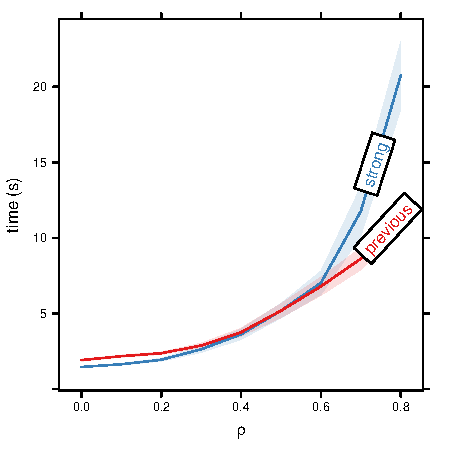
\includegraphics[width=\textwidth]{figures/algorithms.pdf}
            \caption{Performance of strong and previous set strategies for 
                     OLS problems with varying correlation between predictors.}
        \end{figure}
    \end{column}
\end{columns}
\end{frame}

\begin{frame}{Limitations}
\begin{itemize}
    \item the unit slope bound is generally very conservative
    \item does not use second-order structure in any way
    \item current methods for solving SLOPE (FISTA, ADMM) do not make as good use of
          screening rules as coordinate descent does (for the lasso)
\end{itemize}
\end{frame}

\begin{frame}{The SLOPE package for R}

Strong screening rule for SLOPE has been implemented in the R package
SLOPE (\url{https://CRAN.R-project.org/package=SLOPE}). \medskip

Features include
\begin{itemize}
    \item OLS, logistic, Poisson, and multinomial models
    \item support for sparse and dense predictors
    \item cross-validation
    \item efficient codebase in \pkg{C++}
\end{itemize}
\begin{columns}[T]
\begin{column}{0.65\linewidth}
Also have a Google Summer of Code student involved in implementing
proximal Newton solver for SLOPE this summer.
\end{column}
\begin{column}{0.25\linewidth}
\begin{center}

\includegraphics[width=\linewidth]{figures/logo.pdf}
\end{center}
\end{column}
\end{columns}
\end{frame}



\begin{frame}[allowframebreaks]{References}
  \bibliographytrue
  \printbibliography[heading=none]
\end{frame}

\end{document}
